B.2: Arduino Uno 
\label{UcuncuBolum}


	Geliştirilen birçok projede kullanılan en popüler devre kartıdır. Üzerinde birkaç donanım barındırmaktadır. Bunlar: Atmega328 mikrodenetleyici, 16 MHz kristal, güç regülatörü, USB bağlantı portu, gibi bileşenler bulunuyor. Üzerindeki USB dönüştürücü sayesinde hem gerekli kodlar aktarılabilmekte hem de bilgisayar ile iletişim kurulabilmektedir. Kart, üzerindeki fiş jakı sayesinde adaptör tarafından veya üzerindeki USB portu sayesinde kurulan USB bağlantısı tarafından beslenebilmektedir. Arduino Uno kartının ön ve arka görünümü sırasıyla, Şekil 2 ve Şekil 3'de gösterilmiştir.

\begin{figure}[H]
	\centering
	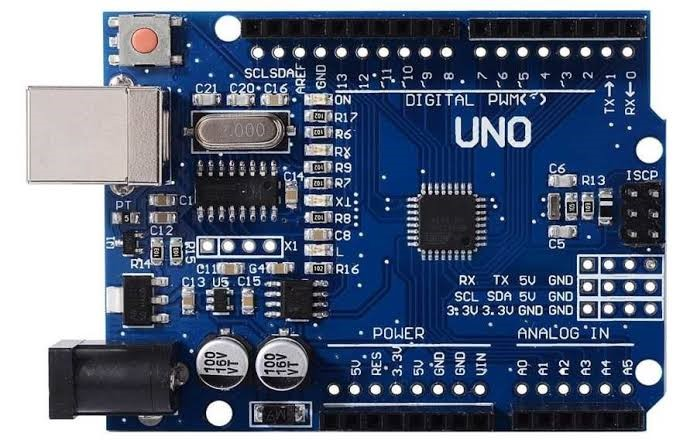
\includegraphics[width=80mm]{grafik/ArduinoOnden.jpg}
    \caption{Arduino Uno (Klon) kartının ön görünümü}
	\label{fig:ArduinoOndenDM}
\end{figure}
\begin{figure}[H]
	\centering
	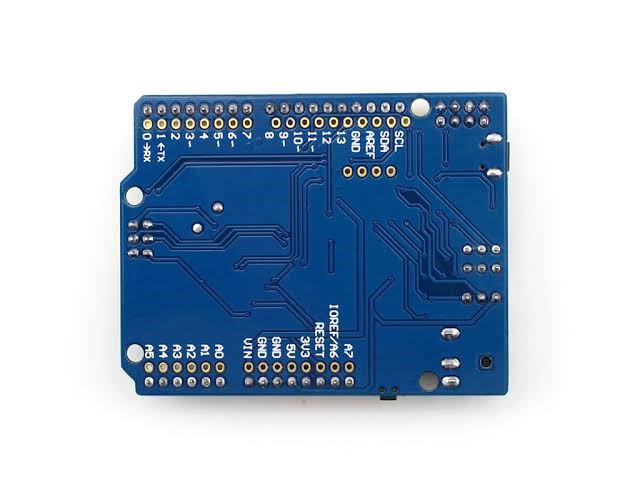
\includegraphics[width=100mm]{grafik/ArduinoArkadan.jpg}
    \caption{Arduino Uno (Klon) kartının arka görünümü}
	\label{fig:ArduinoArkadanDM}
\end{figure}

\clearpage